\ifx\wholebook\relax \else

\documentclass{ctexart}
\usepackage[nomarginpar
  %, margin=.5in
]{geometry}

\addtolength{\oddsidemargin}{-0.05in}
\addtolength{\evensidemargin}{-0.05in}
\addtolength{\textwidth}{0.1in}
\usepackage[cn]{../../../prelude}

\setcounter{page}{1}

\begin{document}

\title{B树}

\author{刘新宇
\thanks{{\bfseries 刘新宇 } \newline
  Email: liuxinyu95@gmail.com \newline}
  }

\maketitle
\fi

\markboth{B树}{基本算法}

\ifx\wholebook\relax
\chapter{B树}
\numberwithin{Exercise}{chapter}
\fi

\section{简介}
\index{B树}
\label{introduction}

上一章介绍的整数前缀树利用二叉树的边来表达信息。另一种扩展二叉树的方法是将分枝的数目从2增加到$k$。B树是一种自平衡的$k$叉搜索树\cite{wiki-b-tree}。它被广泛用于计算机文件系统(基于B+树,一种B树的扩展形势)和数据库系统。图\ref{fig:btree-example}展示了一棵B树,我们可以观察它和二叉搜索树之间的异同。

\begin{figure}[htbp]
  \centering
  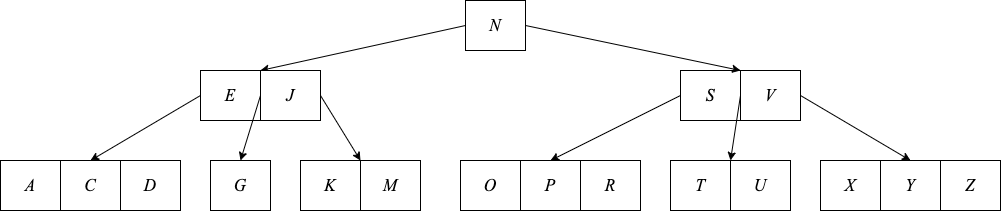
\includegraphics[scale=0.33]{img/btree-del-before.png}
  \caption{B树}
  \label{fig:btree-example}
\end{figure}

一棵二叉搜索树或者为空,或者包含一个元素$k$和左右分枝$l$、$r$。左子树$l$中的任何元素都小于$k$,并且$k$小于右子树$r$中的任何元素\footnote{严格来说,节点中可以保存键(key)和对应的值(value)。值不是必需的。简单起见,本章忽略了节点中的值,称树中保存的内容为“元素”。}:

对于非空的二叉树$(L, k, R)$,其中$L$、$R$和$k$分别代表左右子树和元素。若函数$Key(T)$可以获取树$T$的元素,这一限制条件可以表示为如下形式:

\be
\forall\ x \in l, y \in r \Rightarrow x < k < y
\ee

B树将这一思想推广到多个元素和分枝。一棵B树或者为空,括者包含$n$个元素和$n + 1$个子分枝,每个分枝也都是一棵B树。记这些元素为$k_1, k_2, ..., k_n$,分枝为$t_1, t_2, ..., t_n, t_{n+1}$,如图\ref{fig:btree-node}所示:

\begin{figure}[htbp]
  \centering
  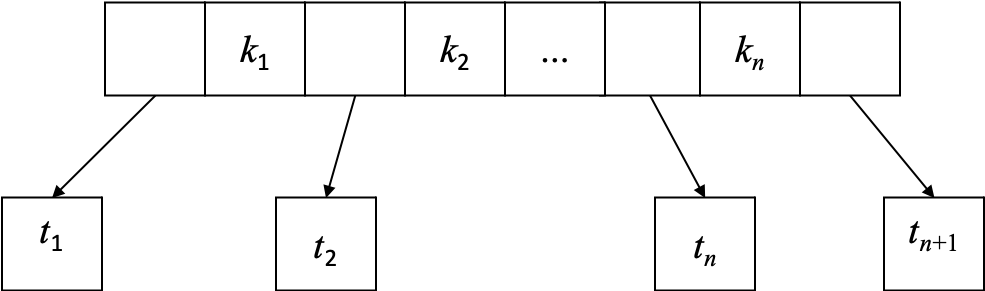
\includegraphics[scale=0.5]{img/btree-node.png}
  \caption{B树节点}
  \label{fig:btree-node}
\end{figure}

节点中的元素和分枝满足以下条件:

\begin{itemize}
\item 元素是递增的:$k_1 \leq k_2 \leq ... \leq k_n$;
\item 对于任意$k_i$,子树$t_i$中的所有元素都小于$k_i$,并且$k_i$小于子树$t_{i+1}$的任意元素。
\end{itemize}

\begin{equation}
\forall\ x_i \in t_i, i=0, 1, ..., n\ \Rightarrow x_1 < k_1 < x_2 < k_2 < ... < x_n < k_n < x_{n+1}
\label{eq:btree-order}
\end{equation}

叶子节点不包含子分枝。令元素的类型为$K$,则B树的类型为$BTree\ K$或\texttt{BTree<K>}。此外,我们还需定义一组规则以保持B树平衡:

\begin{itemize}
\item 所有的叶子节点都有相同的深度;
\item 定义整数$d$,称为B树的\underline{最小度数},每个节点:
    \begin{itemize}
        \item 最多含有$2d - 1$个元素;
        \item 最少含有$d - 1$个元素,根节点例外。
    \end{itemize}
\end{itemize}

即:

\be
  d - 1 \leq |keys(t)|  \leq 2d - 1
\ee

我们接下来证明这些规则使得B树是平衡的。

\begin{proof}
考虑一棵含有$n$个元素的B树,最小度数$d \geq 2$,树的高度为$h$。除根节点外,其它节点至少含有$d - 1$个元素。根节点至少含有一个元素。如果它有子分枝,则至少有两个深度为1的子分枝,至少有$2d$个深度为2的子分枝,至少有$2d^2$个深度为3的子分枝……最后,至少有$2d^{h-1}$个深度为$h$的叶子节点。除根节点外,将节点个数乘以$d - 1$,B树中存储的元素个数满足下面的不等式:

\be
\begin{array}{rl}
n & \geq 1 + (d - 1)(2 + 2d + 2d^2 + ... + 2d^{h-1}) \\
  & = 1 + 2(d - 1) \displaystyle \sum_{k=0}^{h-1} d^k \\
  & = 1 + 2(d - 1) \displaystyle \frac{d^h-1}{d-1} \\
  & = 2d^h - 1
\end{array}
\ee

因此树的高度满足对数关系不等式:

\be
h \leq \log_d \frac{n+1}{2}
\ee

\end{proof}

这就证明了B树的平衡性。最简单的B树称为2-3-4树。它的最小度数$d = 2$,除根节点外的任何节点都包含2到4棵子分枝。任何红黑树本质上都可以转换为一棵2-3-4树。我们记度数为$d$的非空B树为$(d, (ks, ts))$,其中$ks$是元素列表,$ts$是子树列表。下面的例子程序定义了B树:

\lstset{frame = single}
\begin{Haskell}
data BTree a = BTree [a] [BTree a]
\end{Haskell}

空节点记为$(\nil, \nil)$或\texttt{BTree [] []},为了避免在每个节点中都存储一份$d$,我们将其和B树$t$组成一对值$(d, t)$。

\section{插入}
\index{B树!插入} \label{btree-insertion}

插入的思路和二叉搜索树类似,只不过需要面对多个元素和分枝。当向B树$t$插入元素$x$时,我们从根节点开始,查找这样的位置:所有左侧的元素都小于$x$,而右侧的元素大于$x$\footnote{实际上,元素只需支持小于比较和等于比较。参见练习题\ref{ex:btree-leq}。}。如果是未满的叶子节点($|keys(t)| < 2d - 1$),就将$x$插入到此位置。否则,这一位置会指向一棵子树$t'$,我们递归地将$x$插入到$t'$。

\begin{figure}[htbp]
  \centering
  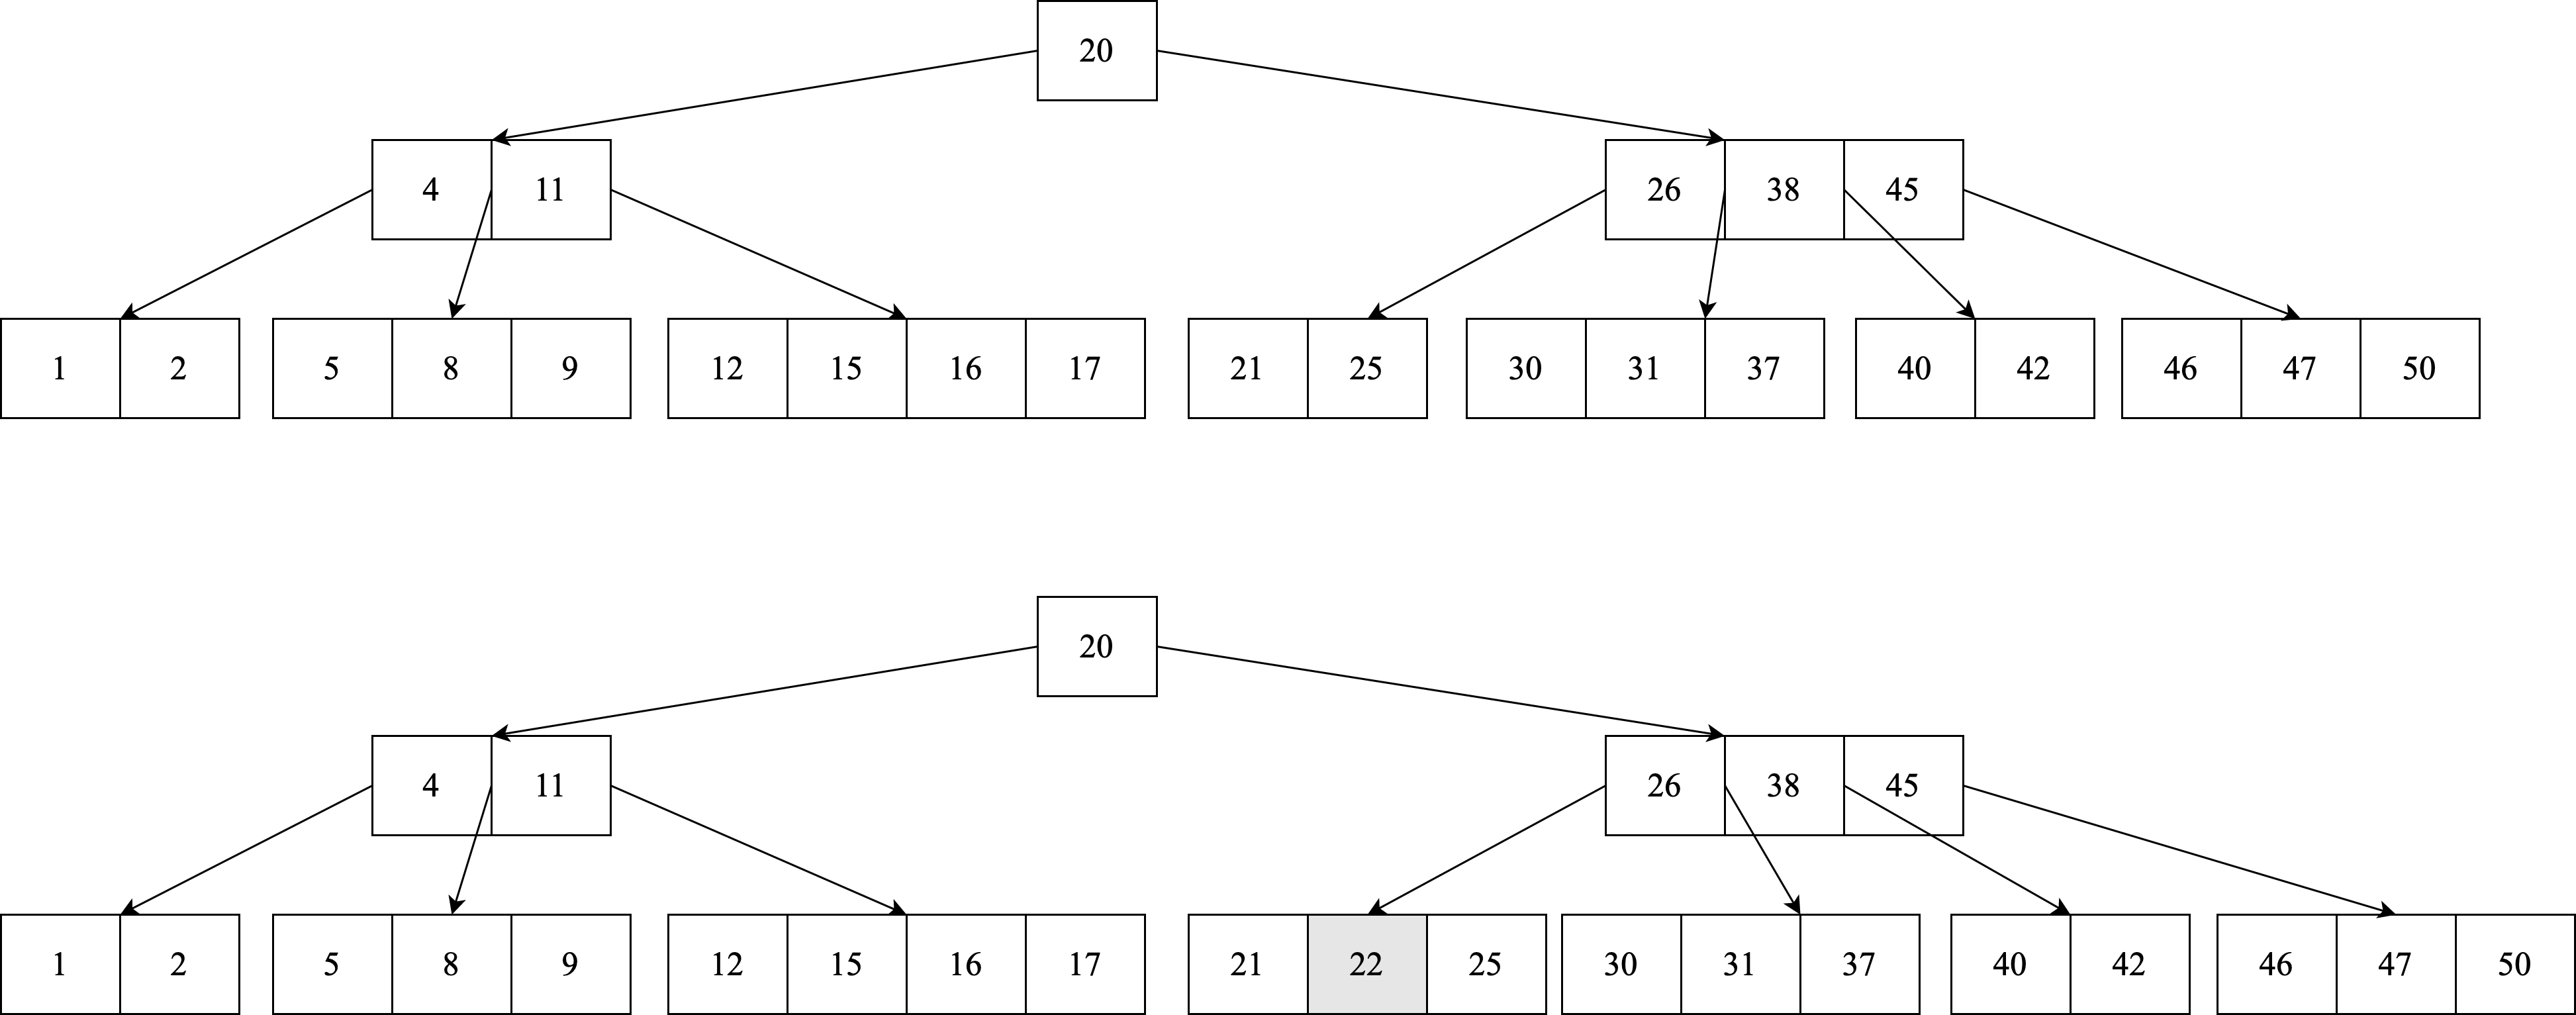
\includegraphics[scale=0.4]{img/btree-insert-example.png}
  \caption{将22插入到2-3-4树:$22 > 20$,插入右子树;$22 < 26$,插入第一棵子树。$21 < 22 < 25$,插入到未满的叶子节点。}
  \label{fig:btree-insert-simple}
\end{figure}

考虑向图\ref{fig:btree-insert-simple}中的2-3-4树插入元素$x = 22$。因为$20 < 22$,我们转向右侧的子树。它包含26、38、45。因为$22 < 26$,所以接下来转向第一棵子树。它包含21和25。这是一个未满的叶子节点,将22插入到21和25中间。

但如果叶子节点中已经含有$2d - 1$个元素,插入$x$后就会因为过多的元素破坏B树的规则。例如向图\ref{fig:btree-insert-simple}插入18就会遇到这个问题。我们有两种解法。

\subsection{先插入再分拆}

我们可以将红黑树中的“先插入再修复”方法扩展到B树。我们先不考虑B树的平衡性,将元素插入到适当的位置。接下来,如果树不再平衡了,我们自下而上对含有过多元素的节点进行分拆。首先我们需要定义函数,用以判断节点是否含有过多或过少的元素。

\be
\begin{cases}
full\ d\ (ks, ts) & = |ks| > 2d - 1 \\
low\  d\ (ks, ts) & = |ks| < d - 1 \\
\end{cases}
\ee

如果含有过多元素和分枝,我们定义$split$函数将其在位置$m$分拆为三部分,如图\ref{fig:node-spilt}所示:

\begin{figure}[htbp]
  \centering
  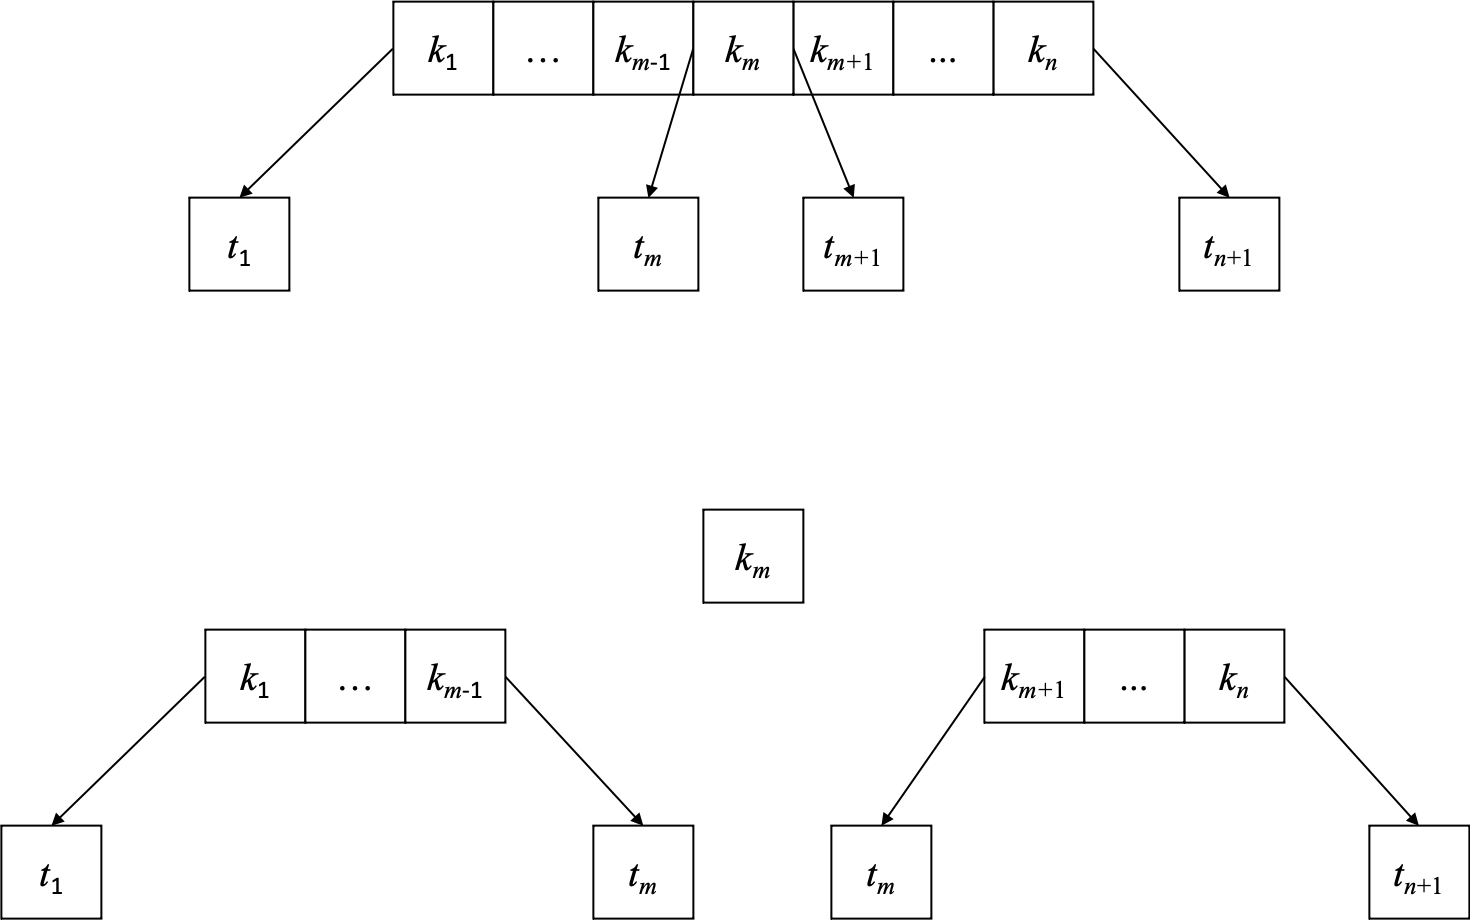
\includegraphics[scale=0.4]{img/split.png}
  \caption{在位置$m$将节点分拆为三部分。}
  \label{fig:node-split}
\end{figure}

\be
split\ m\ (ks, ts) = ((ks_l, ts_l), k, (ks_r, ts_r))
\ee

我们使用第一章(\autoref{eq:split-at})中定义的$splitAt$函数来实现:

\[
\begin{cases}
(ks_l, (k:ks_r)) & = splitAt\ (m - 1)\ ks \\
(ts_l, ts_r) & = splitAt\ m\ ts
\end{cases}
\]

对称地,我们可以定义$unsplit$函数,将三个部分合并成一个B树节点:

\be
unsplit\ (ks_l, ts_l)\ k\ (ks_r, ts_r) = (ks_l \doubleplus [k] \doubleplus ks_r, ts_l \doubleplus ts_r)
\label{eq:btree-unsplit}
\ee

下面的函数先将$x$插入树$t$,然后使用$fix$修复平衡,使得其成为度数为$d$的合法B树:

\be
insert\ x\ (d, t) = fix\ (d, ins\ t)
\ee

在$ins$之后,如果根节点含有过多的元素,函数$fix$使用$split$将其分拆,并构建新的根节点。

\be
fix\ (d, t) = \begin{cases}
  full\ d\ t : & (d, ([k], [l, r])), \text{where}\ (l, k, r) = split\ d\ t \\
  otherwise  : & (d, t)
\end{cases}
\ee

函数$ins$需要处理两种情况:对于叶子节点,我们可以重用第一章(\autoref{eq:list-ordered-insert})定义的列表插入函数$insert$来处理;否则,我们需要找到合适的位置,递归地向子分枝插入。为此,我们定义函数$partition$:

\be
partition\ x\ (ks, ts) = (l, t', r)
\ee

其中$l = (ks_l, ts_l)$、$r = (ks_r, ts_r)$。它进一步使用第一章(\autoref{eq:span})中定义的列表函数$span$进行划分:

\[
\begin{cases}
(ks_l, ks_r) & = span\ (< x)\ ks \\
(ts_l, (t':ts_r)) & = splitAt\ |ks_l|\ ts
\end{cases}
\]

这样,所有小于$x$的元素和所在的子分枝都在左侧$l$,所有大于$x$的都在右侧$r$。我们将最后一棵小于$x$的子分枝取出作为$t'$。接下来我们递归地将$x$插入到$t'$中,如图\ref{fig:recursive-insert}所示。

\be
\begin{array}{rcll}
  ins\ (ks, \nil) & = & (insert_L\ x\ ks, \nil) & \text{列表插入叶子节点}\\
  ins\ (ks, ts)   & = & balance\ d\ l\ (ins\ t')\ r & \text{where}\ (l, t', r) = partition\ x\ t \\
\end{array}
\ee

\begin{figure}[htbp]
  \centering
  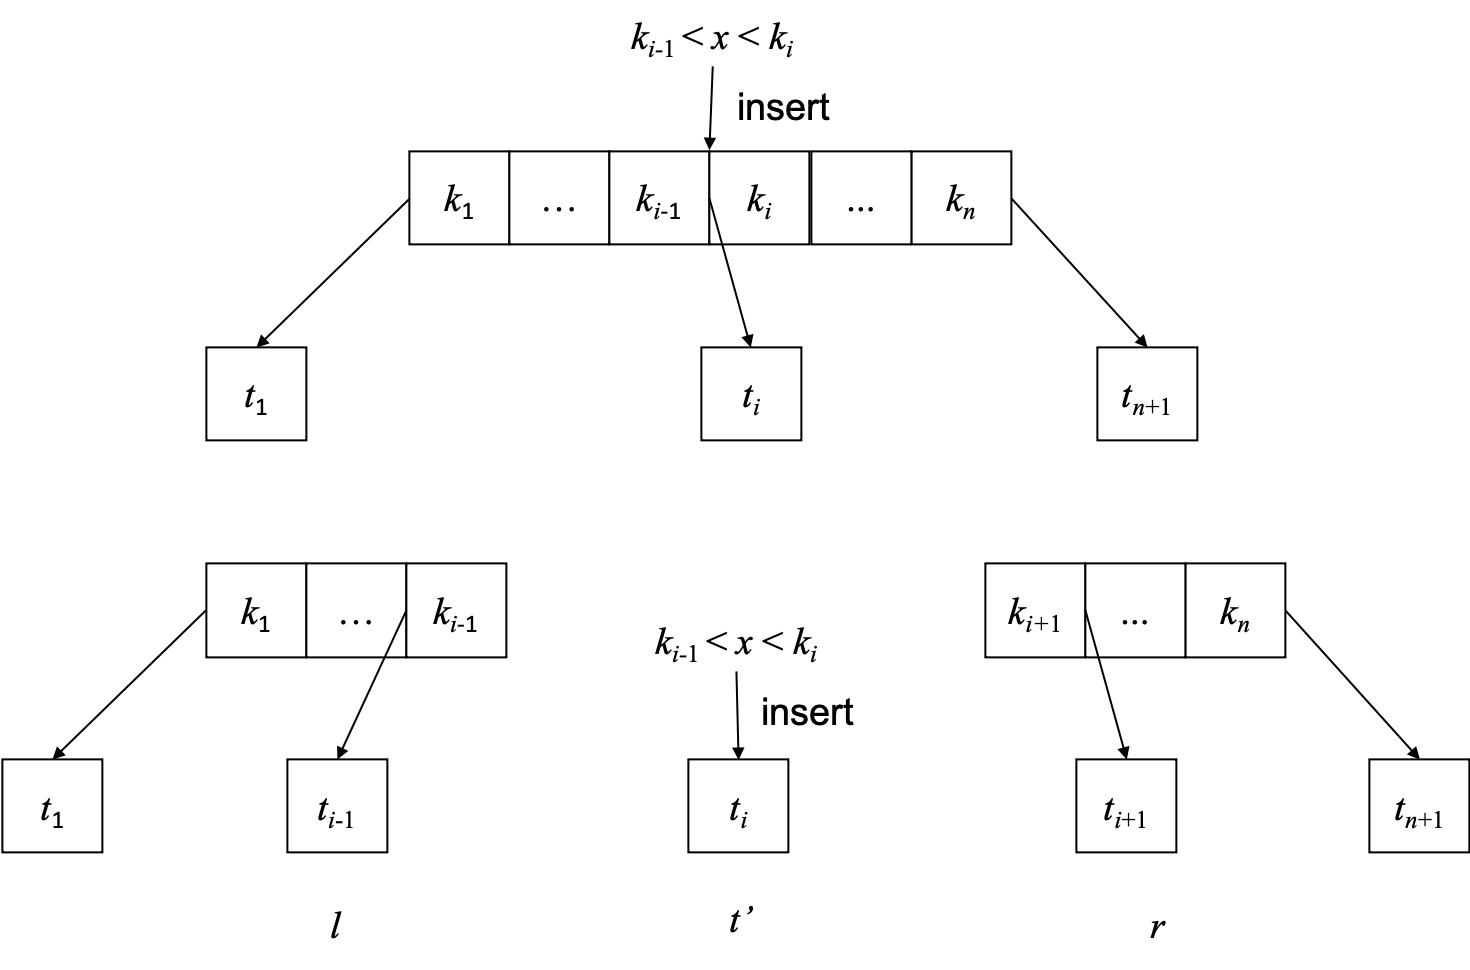
\includegraphics[scale=0.45]{img/partition.png}
  \caption{用$x$划分节点}
  \label{fig:recursive-insert}
\end{figure}

向$t'$插入$x$后,它可能包含来过多的元素,不再满足B树的平衡条件。我们定义函数$balance$来递归地进行分拆修复。

\be
balance\ d\ (ks_l, ts_l)\ t\ (ks_r, ts_r) = \begin{cases}
  full\ d\ t: fix_f \\
  otherwise: (ks_l \doubleplus ks_r, ts_l \doubleplus [t] \doubleplus ts_r)
  \end{cases}
\ee

其中$fix_f$将度数为$d$的子分枝$t$分拆为$(t_1, k, t_2) = split\ d\ t$,然后构建一个新的B树节点:

\be
fix_f = (ks_l \doubleplus [k] \doubleplus ks_r, ts_l \doubleplus [t_1, t_2] \doubleplus ts_r)
\ee

下面的例子程序实现了B树的插入算法:

\begin{Haskell}
partition x (BTree ks ts) = (l, t, r) where
  l = (ks1, ts1)
  r = (ks2, ts2)
  (ks1, ks2) = span (< x) ks
  (ts1, (t:ts2)) = splitAt (length ks1) ts

split d (BTree ks ts) = (BTree ks1 ts1, k, BTree ks2 ts2) where
  (ks1, k:ks2) = splitAt (d - 1) ks
  (ts1, ts2) = splitAt d ts

insert x (d, t) = fixRoot (d, ins t) where
    ins (BTree ks []) = BTree (List.insert x ks) []
    ins t = balance d l (ins t') r where (l, t', r) = partition x t

fixRoot (d, t) | full d t  = let (t1, k, t2) = split d t in
                               (d, BTree [k] [t1, t2])
               | otherwise = (d, t)

balance d (ks1, ts1) t (ks2, ts2)
    | full d t  = fixFull
    | otherwise = BTree (ks1 ++ ks2) (ts1 ++ [t] ++ ts2)
  where
    fixFull = let (t1, k, t2) = split d t in
                BTree (ks1 ++ [k] ++ ks2) (ts1 ++ [t1, t2] ++ ts2)
\end{Haskell}

图\ref{fig:btree-insert-fp}给出了两棵B树的例子,它们都是依次将列表``GMPXACDEJKNORSTUVYZ''中的元素插入B树构造出来的。

\begin{figure}[htbp]
  \centering
  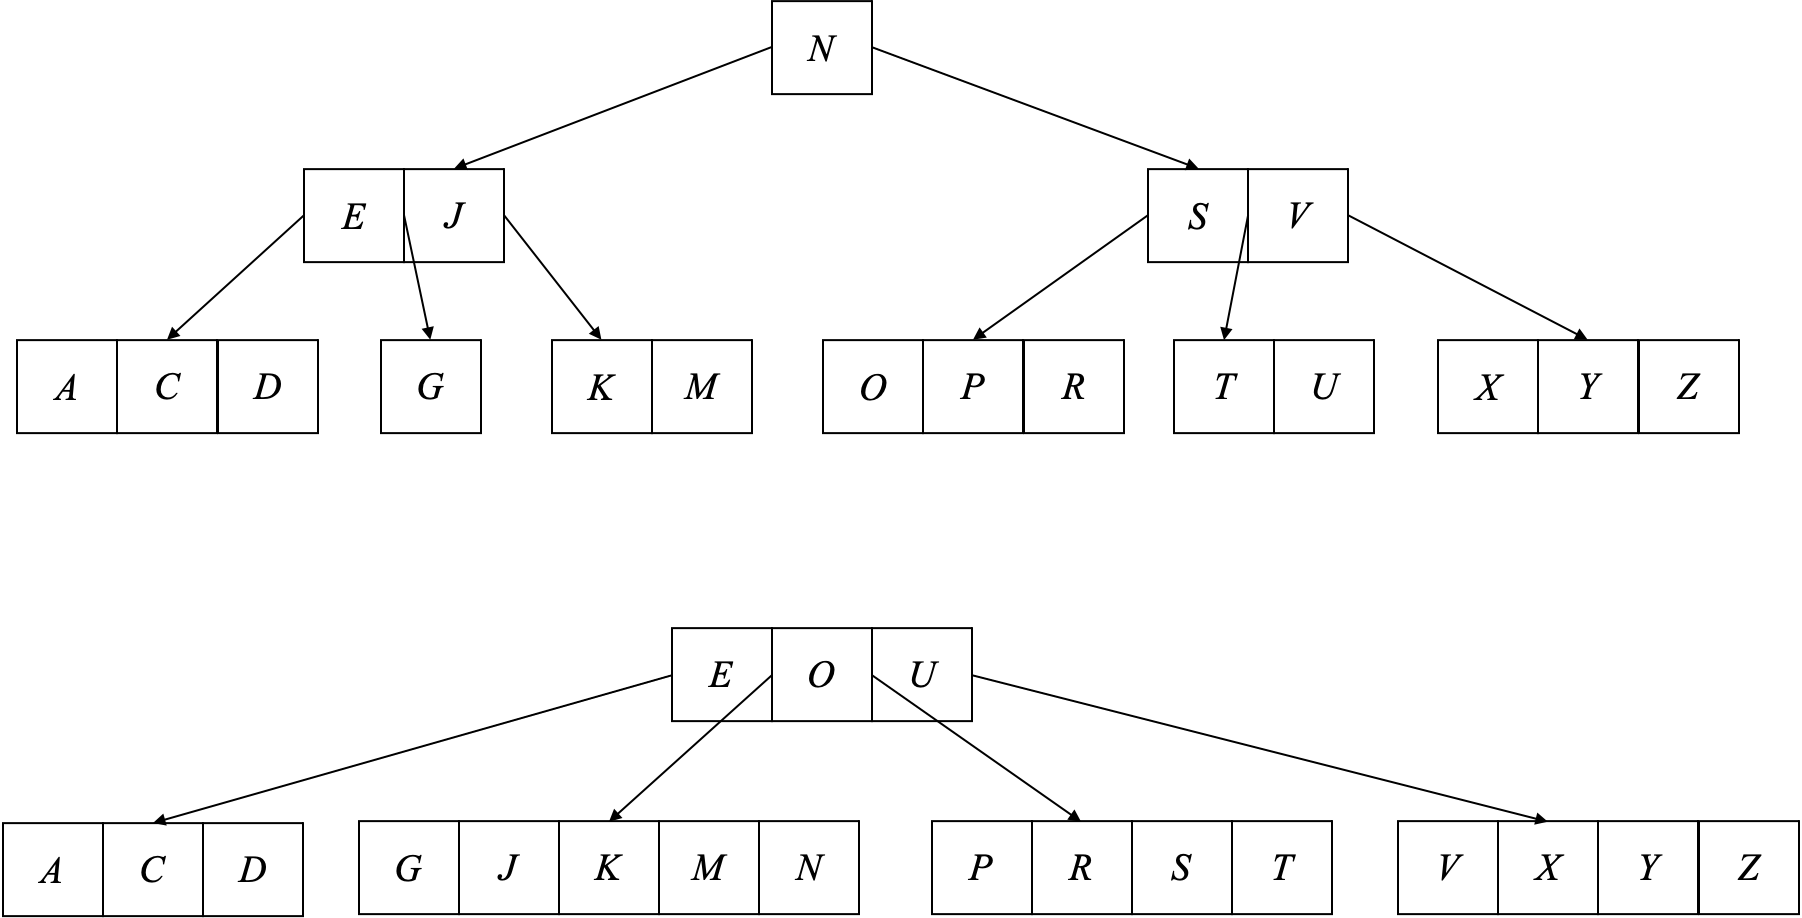
\includegraphics[scale=0.4]{img/btree-insert-fp.png}
  \captionsetup{justification=centering}
  \caption{依次插入``GMPXACDEJKNORSTUVYZ''。\\
上:$d = 2$(2-3-4树),下:$d = 3$}
  \label{fig:btree-insert-fp}
\end{figure}

\subsection{先分拆再插入}

第二种方法是在插入前先分拆节点以避免其含有过多元素。命令式实现常用这一方法。当自顶向下递归插入时,当遇到含有$2d - 1$个元素的节点时,我们将其分拆为三部分,如图\ref{fig:node-split}所示。每个新节点都只含有$d - 1$个元素,即使插入元素后也仍然是合法的B树节点。对于节点$x$,令$K(x)$表示它包含的元素,$T(x)$表示它包含的子分枝。记$x$中的第$i$个元素为$k_i(x)$,第$j$棵子分枝为$t_j(x)$。下面的算法在第$i$个位置对节点$z$进行分拆:

\begin{algorithmic}[1]
\Procedure{Split}{$z, i$}
  \State $d \gets$ \Call{Deg}{$z$}
  \State $x \gets t_i(z)$
  \State $y \gets$ \Call{Create-Node}{}
  \State $K(y) \gets [k_{d + 1}(x), k_{d + 2}(x), ..., k_{2d - 1}(x)]$
  \State $K(x) \gets [k_1(x), k_2(x), ..., k_{d-1}(x)]$
  \If{$x$ is not leaf}
    \State $T(y) \gets [t_{d + 1}(x), t_{d + 2}(x), ..., t_{2d}(x)]$
    \State $T(x) \gets [t_1(x), t_2(x), ..., t_d(x)]$
  \EndIf
  \State \Call{Insert-At}{$K(z), i, k_d(x)$}
  \State \Call{Insert-At}{$T(z), i + 1, y$}
\EndProcedure
\end{algorithmic}

分拆节点$x = t_i(z)$时,我们将第$d$个元素$k_d(x)$向上推入父节点$z$。如果$z$已经满了,推入元素后就会违反B树的规则。为此,我们需要从根节点起,自顶向下沿着插入的路径进行检查,分拆所有含有$2d - 1$个元素的节点。因为所有的父节点都这样被处理过,所以可以接受推上来的元素。这一方法只需要一轮自顶向下的处理,而无需回溯。如果根节点已满,则需要新建一个节点,并将原来的根节点作为它唯一的一棵子树。下面是插入算法的实现:

\begin{algorithmic}[1]
\Function{Insert}{$t, k$}
  \State $r \gets t$
  \If{$r$ is full} \Comment{根节点已满}
    \State $s \gets$ \Call{CREATE-NODE}{}
    \State $T(s) \gets [ r ]$
    \State \Call{Split}{$s, 1$}
    \State $r \gets s$
  \EndIf
  \State \Return \Call{Insert-Nonfull}{$r, k$}
\EndFunction
\end{algorithmic}

其中算法\textproc{Insert-Nonfull}假设传入的节点$r$不满。如果$r$是叶子节点,我们将$k$按照其大小插入到相应的位置(练习\ref{ex:btree-binary-search}要求使用二分查找进行插入)。否则,我们找到一个位置,使得$k_i(r) < k < k_{i+1}(r)$,如果分枝$t_i(r)$满了,就进行分拆。然后继续向子分枝插入。

\begin{algorithmic}[1]
\Function{Insert-Nonfull}{$r, k$}
  \State $n \gets |K(r)|$
  \If{$r$ is leaf}
    \State $i \gets 1$
    \While{$i \leq n$ and $k > k_i(r)$}
      \State $i \gets i + 1$
    \EndWhile
    \State \Call{Insert-At}{$K(r), i, k$}
  \Else
    \State $i \gets n$
    \While{$i > 1$ and $k < k_i(r)$}
      \State $i \gets i - 1$
    \EndWhile
    \If{$t_i(r)$ is full}
      \State \Call{Split}{$r, i$}
      \If{$k > k_i(r)$}
        \State $i \gets i + 1$
      \EndIf
    \EndIf
    \State \Call{Insert-Nonfull}{$t_i(r), k$}
  \EndIf
  \State \Return $r$
\EndFunction
\end{algorithmic}

这一算法是递归的。练习\ref{ex:btree-loop-insert}要求使用循环消除递归。图\ref{fig:btree-insert}给出了依次插入``GMPXACDEJKNORSTUVYZ''时的结果。

\begin{figure}[htbp]
  \centering
  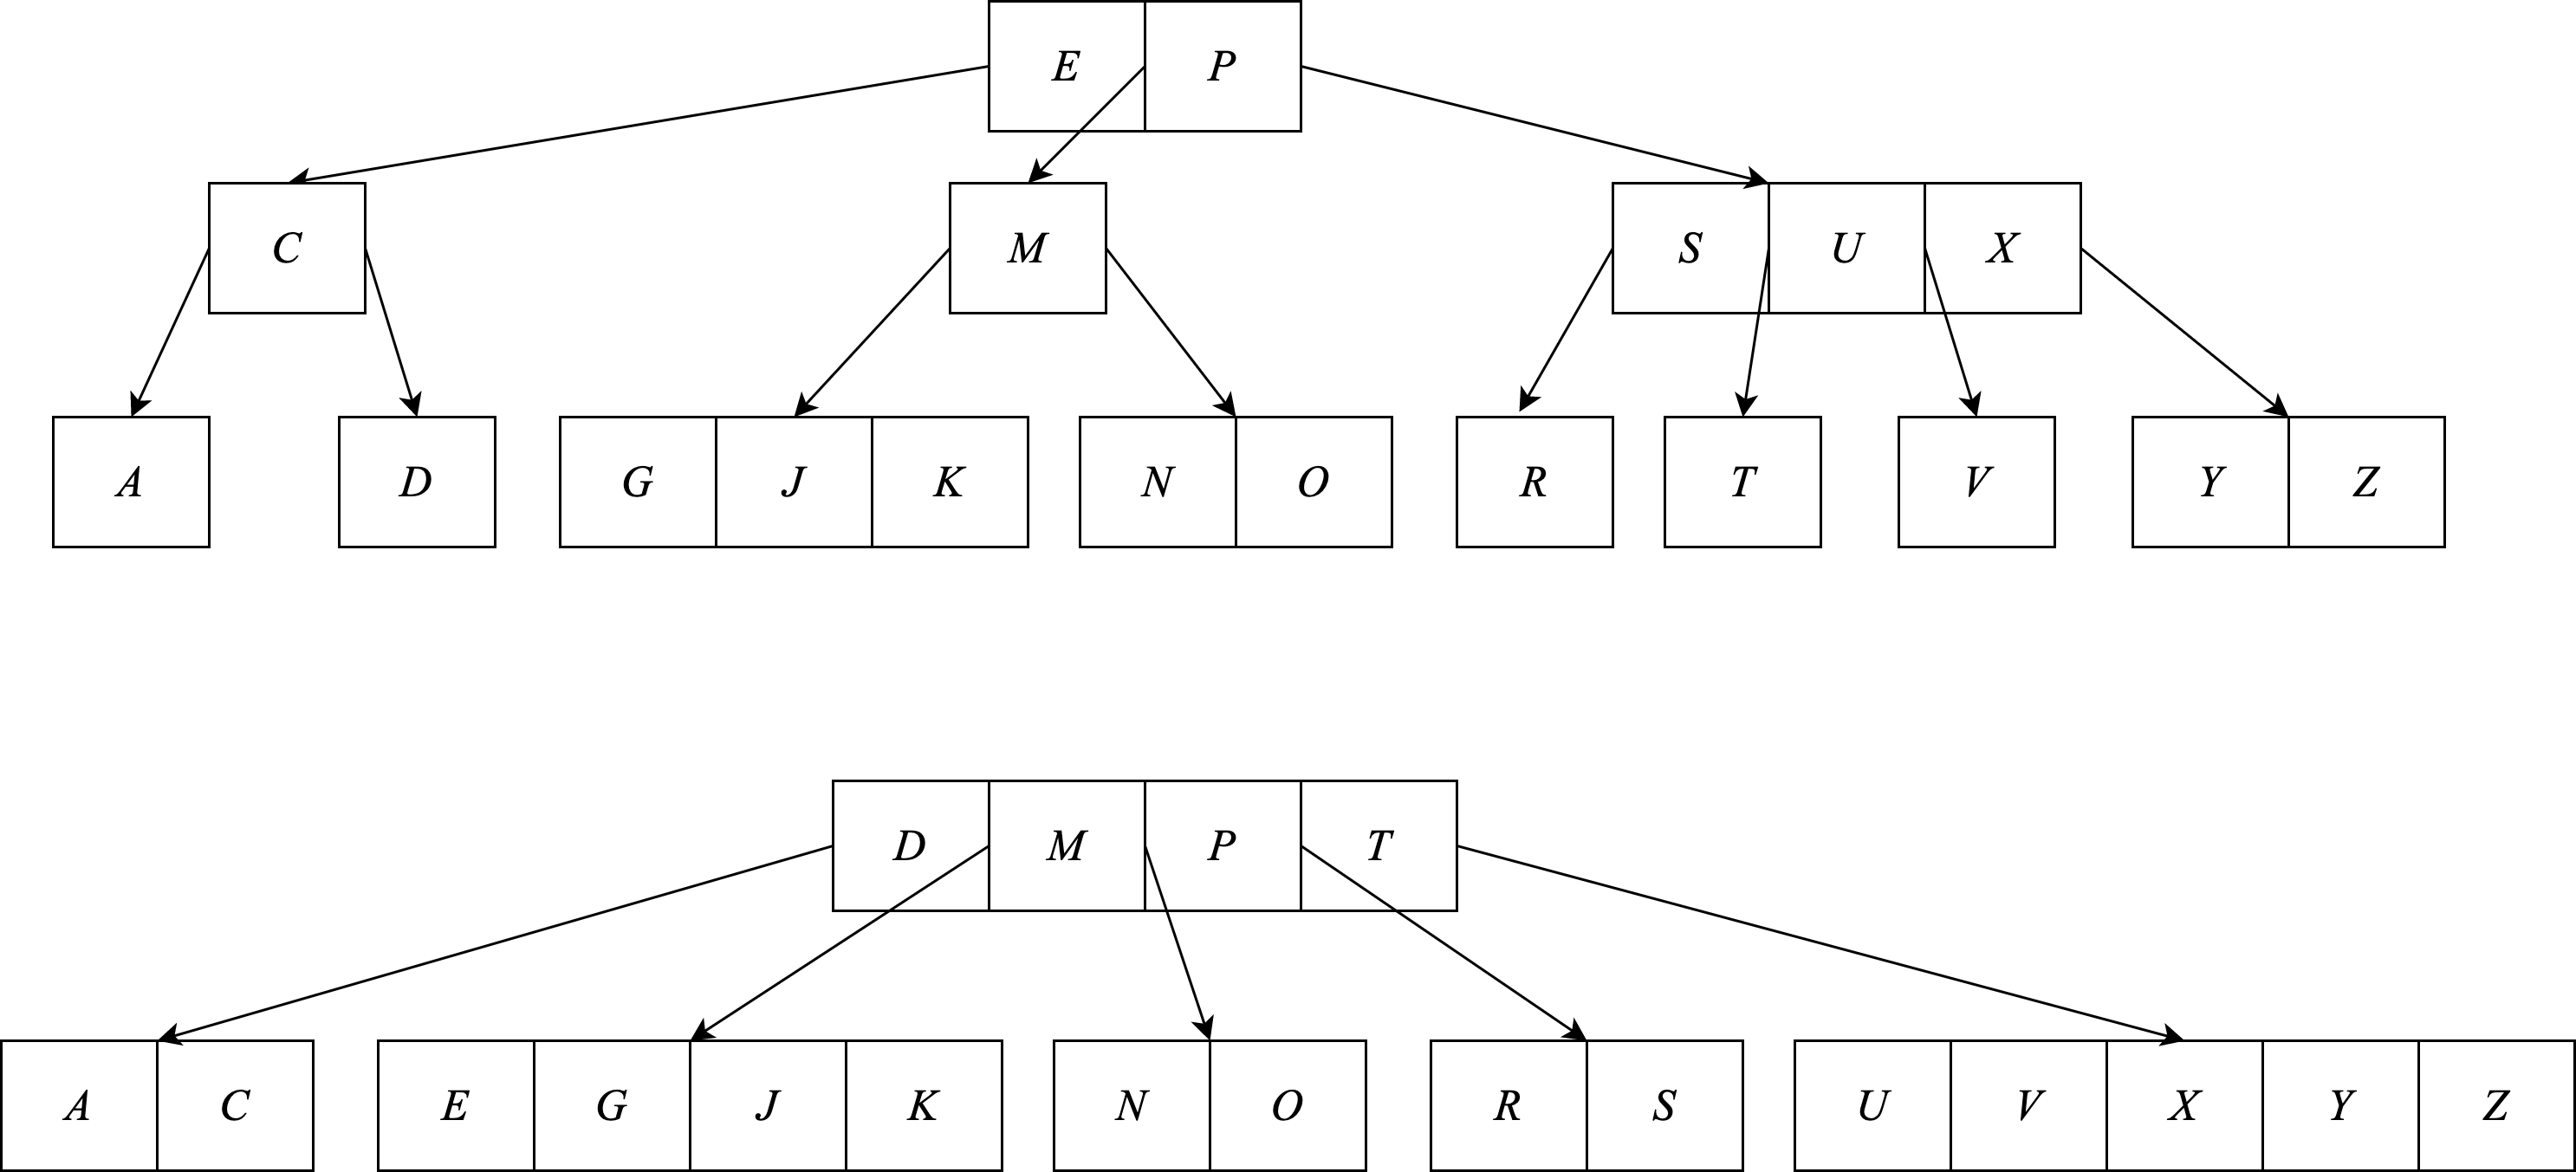
\includegraphics[scale=0.5]{img/btree-split-insert-example.png}
  \caption{依次插入``GMPXACDEJKNORSTUVYZ''。上:$d = 2$(2-3-4树),下:$d = 3$}
  \label{fig:btree-insert}
\end{figure}

\subsection{列表对}

用列表存储元素时,我们需要从第一个元素开始,扫描列表找到插入位置。如果用数组存储,我们可以使用二分查找。可否从节点中的某个位置开始,根据元素的大小向左或向右前进呢?我们可以将B树节点表示为三部分:某棵子分枝$t'$,它的左侧$l$,右侧$r$。其中左右侧都是“元素/子分枝”对$(k_i, t_i)$的列表。特别的,左侧$l$是逆序的。$l$和$r$经由$t'$头对头地连接起来,组成一个如图\ref{fig:paired-lists}所示的马蹄形。我们可以用常数时间前后移动。

\begin{figure}[htbp]
  \centering
  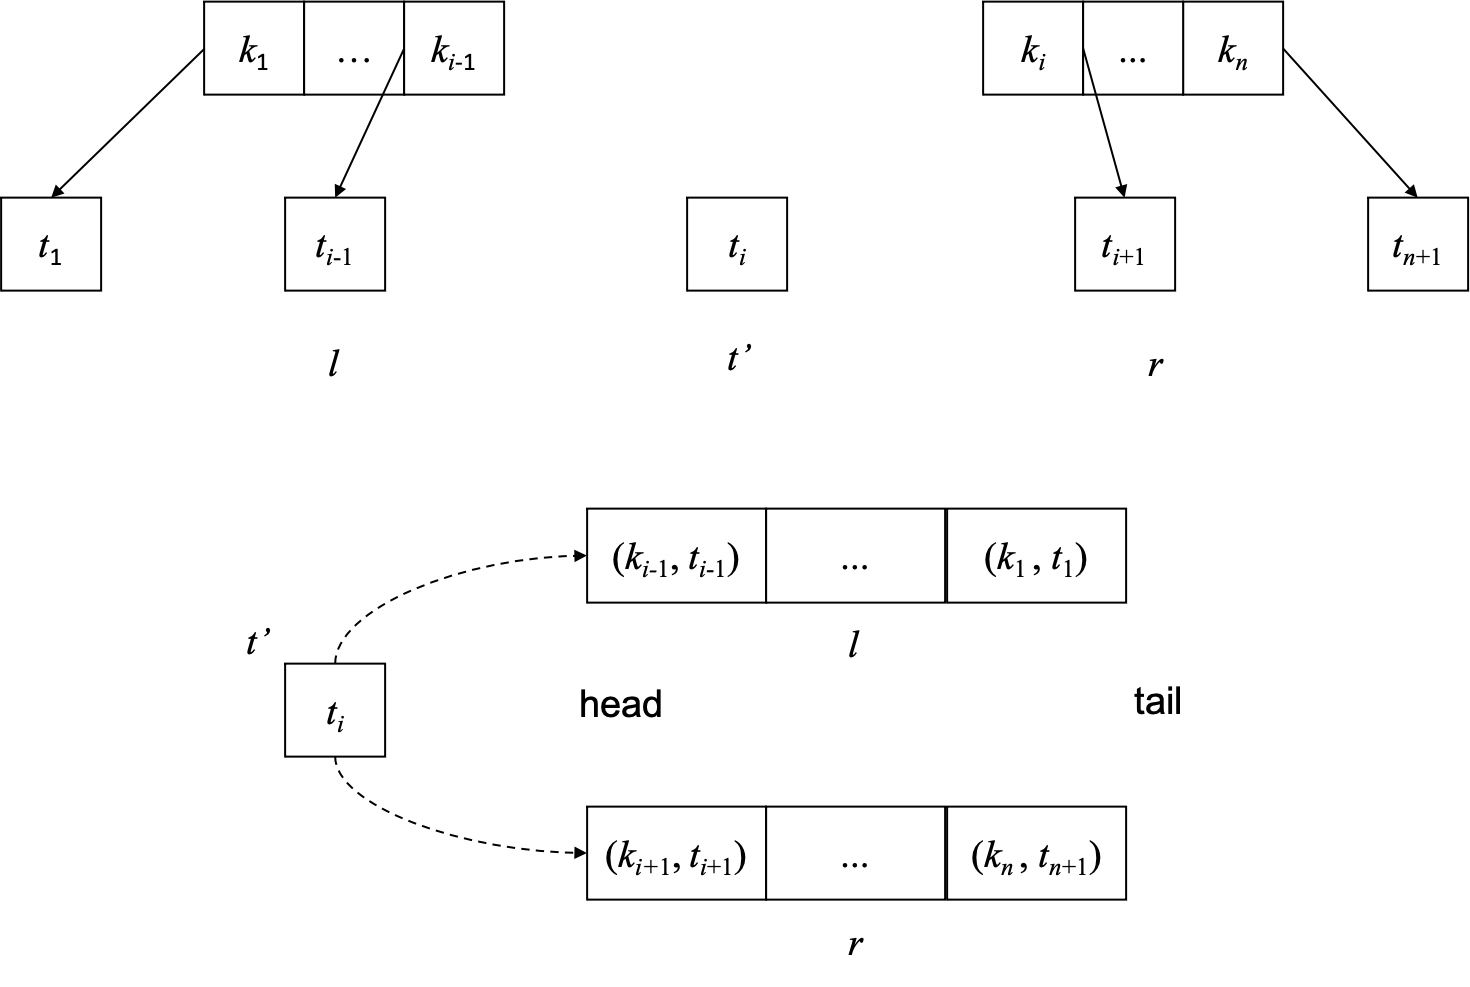
\includegraphics[scale=0.45]{img/paired-lists.png}
  \caption{将B树表示为某个子分枝和它两侧的一对列表}
  \label{fig:paired-lists}
\end{figure}

下面的例子程序用列表对定义了B树节点。它或者为空,或者包含三部分:左侧逆序的(元素,子分枝)列表,中间的某个子分枝,右侧的(元素、子分枝)列表。我们记非空的节点为$(l, t', r)$。

\begin{Haskell}
data BTree a = Empty
           | BTree [(a, BTree a)] (BTree a) [(a, BTree a)]
\end{Haskell}

When move to right by a step, we take the first pair $(k, t)$ from $r$, then form another pair $(k, t')$ in front of $l$, and replace $t'$ with $t$. When move to left a step, it is symmetric. Both operations take constant time.

\be
\begin{array}{lcl}
  step_l\ ((k, t):l, t', r) & = & (l, t, (k, t'):r) \\
  step_r\ (l, t', (k, t):r) & = & ((k, t'):l, t, r) \\
\end{array}
\ee

With the left/right moves, we can implement a generic partition function $partition\ p\ t$, that separates the tree $t$ with a given predicate $p$ into 3 parts: left, middle, right: $(l, m, r)$, such that all sub-trees in $l$ and $m$ satisfy $p$, while the sub-trees in $r$ do not. Let the function $hd = fst \circ head$, which picks the first pair $(a, b)$ from a list, then extracts $a$ out.

\be
\begin{array}{lcl}
  partition\ p\ ([], m, r) & = & \begin{cases}
    p(hd(r)): & partition\ p\ (step_r\ t) \\
    otherwise: & ([], m, r) \\
  \end{cases} \\
  partition\ p\ (l, m, []) & = & \begin{cases}
    (not \circ p)(hd(l)): & partition\ p\ (step_l\ t) \\
    otherwise: & (l, m, []) \\
  \end{cases}\\
  partition\ p\ (l, m, r) & = & \begin{cases}
    p(hd(l))\ \text{and}\ (not \circ p)(hd(r)): & (l, m, r) \\
    p(hd(r)): & partition\ p\ (step_r\ t) \\
    (not \circ p)(hd(l)): & partition\ p\ (step_l\ t) \\
  \end{cases}
\end{array}
\ee

For example, $partition\ (<k)\ t$ moves all keys less than $k$ out of the right part of the tree $t$. Below example program implements the $partition$ function:

\begin{Haskell}
partition p t@(BTree [] m r)
  | p (hd r) = partition p (stepR t)
  | otherwise = ([], m, r)
partition p t@(BTree l m [])
  | (not . p) (hd l) = partition p (stepL t)
  | otherwise = (l, m, [])
partition p t@(BTree l m r)
  | p (hd l) && (not . p) (hd r) = (l, m, r)
  | p (hd r) = partition p (stepR t)
  | (not . p) (hd l) = partition p (stepL t)
\end{Haskell}

We can also use $step_l/step_r$ to split a B-tree at position $d$ when it becomes overly full. Let $n = |l|$ be the number of keys/sub-trees of the left part. $f^n(x)$ means repeatedly apply function $f$ to $x$ for $n$ times.

\be
split\ d\ t = \begin{cases}
  n < d: & sp(step_r^{d - n}(t)) \\
  n > d: & sp(step_r^{n - d}(t)) \\
  otherwise: & sp(t) \\
  \end{cases}
\ee

Where $sp$ does the separation work as below:

\be
sp\ (l, t, (k, t'):r) = ((l, t, []), k, ([], t', r))
\ee

With $partition$ and $split$ defined, we can define B-tree insert algorithm for the paired lists implementation. Firstly, we need modify the low/full testing to count both left and right parts:

\be
\begin{array}{ll}
  full\ d\ \nil & = False \\
  full\ d\ (l, t', r) & = |l| + |r| > 2d - 1 \\
\end{array}
\ee
and
\be
\begin{array}{ll}
  low\  d\ \nil & = False \\
  low\  d\ (l, t', r) & = |l| + |r| < d - 1 \\
\end{array}
\ee

When insert key $x$ to B-tree $t$ of degree $d$, we do the recursive insertion, then fix the root if it gets overly full:

\be
insert\ x\ (d, t) = fix\ (d, ins\ t)
\ee

Where $fix$ splits the root at $d$ if needed:

\be
fix\ (d, t) = \begin{cases}
  full\ d\ t: & (d, ([], t_1, [(k, t_2)]\ \text{where}\ (t_1, k, t_2) = split\ d\ t \\
  otherwise: & (d, t)
  \end{cases}
\ee

Function $ins$ need handle both $t = \nil$, and $t \neq \nil$ cases. For empty case, we create a singleton leaf; otherwise, we call $(l, t', r) = partition\ (< x)\ t$ to locate the position for recursive insert:

\be
\begin{array}{lcl}
  ins\ \nil & = & ([], \nil, [(x, \nil)]) \\
  ins\ t & = & \begin{cases}
    t' = \nil: & balance\ d\ l\ \nil\ ((x, \nil):r) \\
    t' \neq \nil: & balance\ d\ l\ (ins\ t')\ r \\
  \end{cases}
\end{array}
\ee

Function $balance$ examines if the sub-tree $t$ contains too many keys, and splits it.

\be
balance\ d\ l\ t\ r = \begin{cases}
  full\ d\ t: & fixFull \\
  otherwise: & (l, t, r)
  \end{cases}
\ee

Where $fixFull = (l, t_1, ((k, t_2):r)$, and $(t_1, k, t_2) = split\ d\ t$. Below example program implements the insert algorithm:

\begin{Haskell}
insert x (d, t) = fixRoot (d, ins t) where
  ins Empty = BTree [] Empty [(x, Empty)]
  ins t = let (l, t', r) = partition (< x) t in
    case t' of
      Empty -> balance d l Empty ((x, Empty):r)
      _     -> balance d l (ins t') r

fixRoot (d, t) | full d t = let (t1, k, t2) = split d t in
                   (d, BTree [] t1 [(k, t2)])
               | otherwise = (d, t)

balance d l t r | full d t = fixFull
                | otherwise = BTree l t r
  where
    fixFull = let (t1, k, t2) = split d t in BTree l t1 ((k, t2):r)

split d t@(BTree l _ _) | n < d = sp $ iterate stepR t !! (d - n)
                        | n > d = sp $ iterate stepL t !! (n - d)
                        | otherwise = sp t
  where
    n = length l
    sp (BTree l t ((k, t'):r)) = (BTree l t [], k, BTree [] t' r)
\end{Haskell}

\begin{Exercise}
\Question{Can we use $\leq$ to support duplicated keys in B-Tree?} \label{ex:btree-leq}
\Question{For the `split then insert' algorithm, eliminate the recursion with loops.}
\label{ex:btree-loop-insert}
\Question{We use linear search among keys to find the proper insert position. Improve the imperative implementation with binary search. Is the big-O performance improved?}
\label{ex:btree-binary-search}
% No, is still linear, although the search speed up to O(\lg n), the insertion takes O(n) time to shift elements.
\end{Exercise}

% ================================================================
%               Deletion
% ================================================================
\section{删除}
\index{B树!删除}

最小度数为$t$的B树中,除根节点外,任何节点中的key都不能少于$t-1$个。从节点中删除一个key后,有可能会违反这一平衡性质。

同插入操作一样,我们可以采用类似的策略:或者在删除前进行额外的准备工作,以保证节点含有足够多的key;或者在删除后对节点进行修复,以避免含有的key过少。


% ================================================================
%               Merge before delete method
% ================================================================
\subsection{删除前预合并}

我们先处理最简单的情况:如果待删除的key $k$所在的节点为一叶子节点$x$,我们可以直接将$k$从$x$中删除。如果$x$是根节点(树中的唯一节点),我们无需担心删除后含有的key过少。以上两种,我们称之为\underline{情况1}。

通常情况下,我们从根节点开始,自顶向下沿着一条路径定位到$k$所在的节点$x$。如果$x$是一分支节点,则有如下三种子情况:

\begin{itemize}
\item 子情况2a:如果$k$前面的子节点$y$含有足够多的key(多于$t$),我们用$y$中$k$的前驱元素$k'$替换掉$x$中的$k$,然后递归地在$y$中将$k'$删除。

其中,$k$的前驱元素就是子节点$y$中的最后一个key。

图\ref{fig:btree-del-case2a}描述了这种情况。

\begin{figure}[htbp]
  \centering
    \includegraphics[scale=0.5]{img/btree-del-case2a.eps}
    \caption{使用前驱元素替换并递归进行删除} \label{fig:btree-del-case2a}
\end{figure}

\item 子情况2b:如果$y$含有的key不足,但是$k$的后继子节点$z$含有的key多于$t$,我们可以将$x$中的元素$k$用$z$中$k$的后继元素$k''$来替换,然后再递归地将$z$中的$k''$删除。

其中,$k$的后继元素就是子节点$z$中的第一个key。

图\ref{fig:btree-del-case2b}描述了这种情况。

\begin{figure}[htbp]
  \centering
    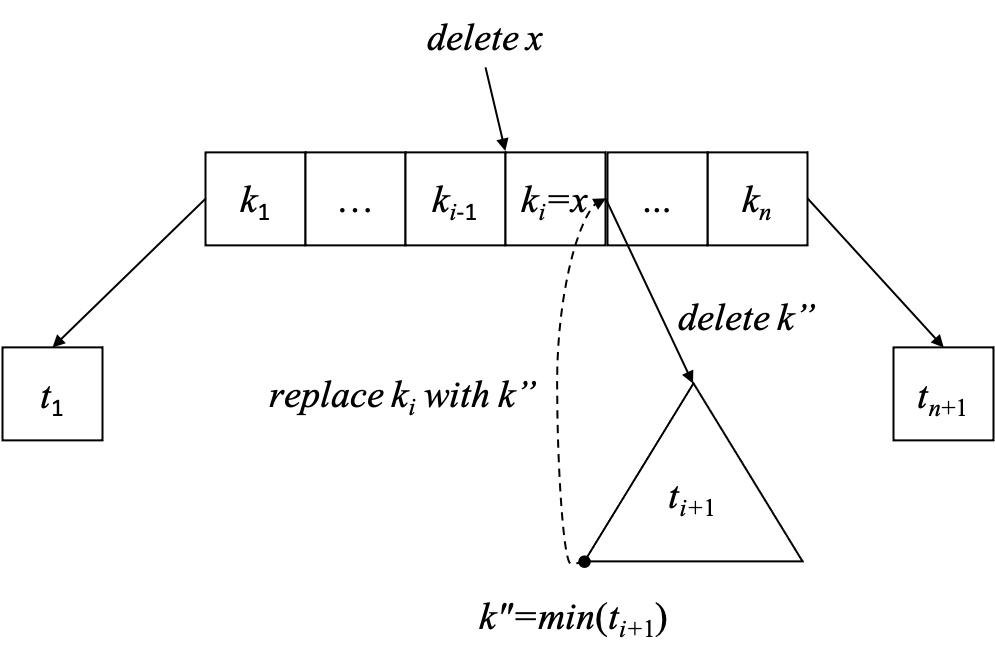
\includegraphics[scale=0.5]{img/btree-del-case2b.eps}
    \caption{使用后继元素替换并递归进行删除} \label{fig:btree-del-case2b}
\end{figure}

\item 子情况2c:否则,如果$y$和$z$含有的key都不足,我们可以将$y$、$k$和$z$合并成一个新节点,它恰好含有$2t-1$个key,此后,我们就可以针对这个新节点进行递归删除。

这里有一个特殊情况:如果合并后的节点不含有任何key,也就是说,$k$是$x$中的唯一key,而$y$和$z$是$x$仅有的两个子节点。这时我们需要将树的高度降低一层。
\end{itemize}

图\ref{fig:btree-del-case2c}描述了这种情况。

\begin{figure}[htbp]
  \centering
    \includegraphics[scale=0.5]{img/btree-del-case2c.eps}
    \caption{合并后再删除} \label{fig:btree-del-case2c}
\end{figure}

还有一种情况,如果$k$不是节点$x$中的key,我们需要在$x$中找到一个子节点$c_i$,使得$k$在子树$c_i$中。在对$c_i$进行递归删除前,我们需要预先确定$c_i$至少含有$t$个key。如果含有的key不足,就需要进行如下的调整。

\begin{itemize}
\item 子情况3a:我们检查$c_i$的前后兄弟节点$c_{i-1}$和$c_{i+1}$。如果任何一个节点包含有足够的key(至少$t$个),我们就将$x$中的一个key向下移动到$c_i$中,并将含有足够多key的兄弟节点中的一个key向上移动到$x$中。同时,我们还需要将兄弟节点中相应的子节点移动到$c_i$中。

这一操作使得$c_i$含有足够多的key以便进行后面的删除。接下来我们可以从$c_i$中递归删除$k$。

图\ref{fig:btree-del-case3a}描述了这一情况。

\begin{figure}[htbp]
  \centering
    \includegraphics[scale=0.5]{img/btree-del-case3a.eps}
    \caption{向右侧的兄弟节点“借”一个key}
    \label{fig:btree-del-case3a}
\end{figure}

\item 子情况3b:如果左右两个兄弟节点含有的key都不足,我们可以将$c_i$,$x$中的一个key,和任一兄弟节点合并为一个新节点。然后针对这一节点执行删除操作。
\end{itemize}

图\ref{fig:btree-del-case3b}描述了这一情况。

\begin{figure}[htbp]
  \centering
    \includegraphics[scale=0.5]{img/btree-del-case3b.eps}
    \caption{将$c_i$、$k$和$c_{i+1}$合并为一个新节点}
    \label{fig:btree-del-case3b}
\end{figure}

为了实现删除算法,我们需要先定义一些辅助函数。函数\textproc{Can-Del}检查一个节点是否含有足够多的key以执行删除操作。

\begin{algorithmic}[1]
\Function{Can-Del}{$T$}
  \State \Return $|K(T)| \ge t$
\EndFunction
\end{algorithmic}

过程\textproc{Merge-Children}($T, i$)将子节点$c_i(T)$、key $k_i(T)$和子节点$c_{i+1}(T)$合并成一个新节点。

\begin{algorithmic}[1]
\Procedure{Merge-Children}{$T, i$} \Comment{将$c_i(T)$、$k_i(T)$和$c_{i+1}(T)$合并}
  \State $x \gets c_i(T)$
  \State $y \gets c_{i+1}(T)$
  \State $K(x) \gets K(x) \cup \{k_i(T)\} \cup K(y)$
  \State $C(x) \gets C(x) \cup C(y)$
  \State \Call{Remove-At}{$K(T), i$}
  \State \Call{Remove-At}{$C(T), i+1$}
\EndProcedure
\end{algorithmic}

这一过程从给定的树$T$中定位到第$i$个子节点和key,将它们和第$i+1$个节点合并,然后从$T$中将第$i$个key和第$i+1$个子节点删除。

使用上述函数,我们可以分别处理三种不同的情况,从而定义下面的B树删除算法。

\begin{algorithmic}[1]
\Function{Delete}{$T, k$}
  \State $i \gets 1$
  \While{$i \leq |K(T)|$}
    \If{$k = k_i(T)$}
      \If{$T$ is leaf} \Comment{情况1}
        \State \Call{Remove}{$K(T), k$}
      \Else \Comment{情况2}
        \If{\Call{Can-Del}{$c_i(T)$}} \Comment{情况2a}
          \State $k_i(T) \gets$ \Call{Last-Key}{$c_i(T)$}
          \State \Call{Delete}{$c_i(T), k_i(T)$}
        \ElsIf{\Call{Can-Del}{$c_{i+1}(T)$}} \Comment{情况2b}
          \State $k_i(T) \gets$ \Call{First-Key}{$c_{i+1}(T)$}
          \State \Call{Delete}{$c_{i+1}(T), k_i(T)$}
        \Else \Comment{情况2c}
          \State \Call{Merge-Children}{$T, i$}
          \State \Call{Delete}{$c_i(T), k$}
          \If{$K(T) = NIL$}
            \State $T \gets c_i(T)$ \Comment{缩小高度}
          \EndIf
        \EndIf
      \EndIf
      \State \Return $T$
    \ElsIf{$k < k_i(T)$}
      \State Break
    \Else
      \State $i \gets i+1$
    \EndIf
  \EndWhile
  \Statex
  \If{$T$ is leaf}
    \State \Return $T$ \Comment{$k$不在$T$中}
  \EndIf
  \If{$\lnot$ \Call{Can-Del}{$c_i(T)$}}  \Comment{情况3}
    \If{$i>1 \land$ \Call{Can-Del}{$c_{i-1}(T)$}} \Comment{情况3a:左侧兄弟}
      \State \Call{Insert}{$K(c_i(T)), k_{i-1}(T)$}
      \State $k_{i-1}(T) \gets$ \Call{Pop-Back}{$K(c_{i-1}(T))$}
      \If{$c_i(T)$ isn't leaf}
        \State $c \gets$ \Call{Pop-Back}{$C(c_{i-1}(T))$}
        \State \Call{Insert}{$C(c_i(T)), c$}
      \EndIf
    \ElsIf{$i \leq |C(T)| \land$ \Call{Can-Del}{$c_{i_1}(T)$}} \Comment{情况3a:右侧兄弟}
      \State \Call{Append}{$K(c_i(T)), k_i(T)$}
      \State $k_i(T) \gets$ \Call{Pop-Front}{$K(c_{i+1}(T))$}
      \If{$c_i(T)$ isn't leaf}
        \State $c \gets$ \Call{Pop-Front}{$C(c_{i+1}(T))$}
        \State \Call{Append}{$C(c_i(T)), c$}
      \EndIf
    \Else \Comment{情况3b}
      \If{$i>1$}
        \State \Call{Merge-Children}{$T, i-1$}
      \Else
        \State \Call{Merge-Children}{$T, i$}
      \EndIf
    \EndIf
  \EndIf
  \State \Call{Delete}{$c_i(T), k$} \Comment {递归删除}
  \If{$K(T) = NIL$} \Comment {缩小高度}
    \State $T \gets c_1(T)$
  \EndIf
  \State \Return $T$
\EndFunction
\end{algorithmic}

图\ref{fig:result-del1}、\ref{fig:result-del2}和\ref{fig:result-del3}描述了删除中的各个步骤,被改变的节点用灰色显示。

\begin{figure}[htbp]
  \centering
  \subcaptionbox{删除前的B树}{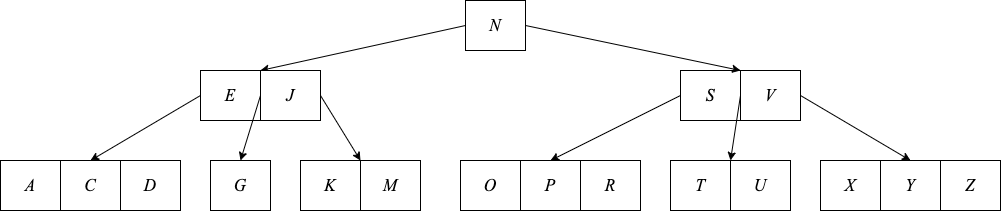
\includegraphics[scale=0.5]{img/btree-del-before.ps}} \\
  \subcaptionbox{删除key ‘F’,情况1}{\includegraphics[scale=0.5]{img/btree-del-F.ps}}
  \caption{B树删除的结果(1)} \label{fig:result-del1}
\end{figure}

\begin{figure}[htbp]
  \centering
  \subcaptionbox{删除key ‘M’后,子情况2a}{\includegraphics[scale=0.5]{img/btree-del-M.ps}} \\
  \subcaptionbox{删除key ‘G’后,子情况2c}{\includegraphics[scale=0.5]{img/btree-del-G.ps}}
  \caption{B树删除的结果(2)} \label{fig:result-del2}
\end{figure}

\begin{figure}[htbp]
  \centering
  \subcaptionbox{删除key ‘D’后,子情况3b,树的高度减少1}{\includegraphics[scale=0.5]{img/btree-del-D.ps}} \\
  \subcaptionbox{删除key ‘B’后,子情况3a,向右侧兄弟节点”借“一个key}{\includegraphics[scale=0.5]{img/btree-del-B.ps}} \\
  \subcaptionbox{删除key ‘U’后,子情况3a,向左侧兄弟节点“借”一个key}{\includegraphics[scale=0.5]{img/btree-del-U.ps}}
  \caption{B树删除的结果(3)} \label{fig:result-del3}
\end{figure}

下面的Python例子程序实现了B树的删除算法。

\lstset{language=Python}
\begin{lstlisting}
def can_remove(tr):
    return len(tr.keys) >= tr.t

def replace_key(tr, i, k):
    tr.keys[i] = k
    return k

def merge_children(tr, i):
    tr.children[i].keys += [tr.keys[i]] + tr.children[i+1].keys
    tr.children[i].children += tr.children[i+1].children
    tr.keys.pop(i)
    tr.children.pop(i+1)

def B_tree_delete(tr, key):
    i = len(tr.keys)
    while i>0:
        if key == tr.keys[i-1]:
            if tr.leaf:  # 情况1
                tr.keys.remove(key)
            else: # 情况2
                if tr.children[i-1].can_remove(): # 情况2a
                    key = tr.replace_key(i-1, tr.children[i-1].keys[-1])
                    B_tree_delete(tr.children[i-1], key)
                elif tr.children[i].can_remove(): # 情况2b
                    key = tr.replace_key(i-1, tr.children[i].keys[0])
                    B_tree_delete(tr.children[i], key)
                else: # 情况2c
                    tr.merge_children(i-1)
                    B_tree_delete(tr.children[i-1], key)
                    if tr.keys==[]: # 缩减树的高度
                        tr = tr.children[i-1]
            return tr
        elif key > tr.keys[i-1]:
            break
        else:
            i = i-1
    # 情况3
    if tr.leaf:
        return tr # key不存在
    if not tr.children[i].can_remove():
        # 情况3a
        if i>0 and tr.children[i-1].can_remove(): # 左侧兄弟
            tr.children[i].keys.insert(0, tr.keys[i-1])
            tr.keys[i-1] = tr.children[i-1].keys.pop()
            if not tr.children[i].leaf:
                tr.children[i].children.insert(0, tr.children[i-1].children.pop())
        elif i<len(tr.children) and tr.children[i+1].can_remove(): # 右侧兄弟
            tr.children[i].keys.append(tr.keys[i])
            tr.keys[i]=tr.children[i+1].keys.pop(0)
            if not tr.children[i].leaf:
                tr.children[i].children.append(tr.children[i+1].children.pop(0))
        else: # 情况3b
            if i>0:
                tr.merge_children(i-1)
            else:
                tr.merge_children(i)
    B_tree_delete(tr.children[i], key)
    if tr.keys==[]: # 缩减树的高度
        tr = tr.children[0]
    return tr
\end{lstlisting}

% ================================================================
%               Delete and fix method
% ================================================================

\subsection{先删除再修复}

删除前预合并算法比较复杂了,需要处理不同的情况,每种情况又含有若干子情况。

我们也可以换一种思路来设计删除算法。即先删除,然后再进行必要的修复。这种策略和先插入再修复相类似。

\be
delete(T, k) = fix(del(T, k))
\ee

从B树删除一个key时,我们先从根节点开始,自顶向下定位到这个key所在的节点。

如果这一节点是一个叶子节点,我们就删掉相应的key,然后检查节点种剩余的key是否太少以至于无法满足B树的平衡条件。

如果这一节点是一个分支节点,删掉key后它就被分为两部分。我们合并它们。这一合并过程是递归的,如图\ref{fig:del-fp-merge}所示。

\begin{figure}[htbp]
  \centering
  \includegraphics[scale=0.5]{img/btree-del-fp-merge.eps}
  \caption{从分支节点种删除key。删除$k_i$后节点分成了两部分。递归将它们合并直到这两部分都是叶子节点。} \label{fig:del-fp-merge}
\end{figure}

合并时,如果待合并的两个节点不是叶子节点,我们将key合到一起,然后递归地将左侧部分的最后一个子树和右侧部分的第一个子树合并。否则,如果它们都是叶子节点,我们只需要将key合并到一起。

到目前为止,待删除的key已经从树中去掉了。但是由此导致节点中key的减少可能会违反B树的平衡条件。我们需要从根节点开始,沿着删除时经过的路径进行修复。

\begin{figure}[htbp]
  \centering
  \includegraphics[scale=0.5]{img/btree-del-fp-make.eps}
  \caption{从节点$c_i$中删除key $k$后,结果为$c_i'$。修复时,我们用左侧部分、$c_i'$和右侧部分构造一个新节点。}
  \label{fig:del-fp-make}
\end{figure}

经过递归删除,路径上的任何一个分支节点都被分成了三部分:左侧部分包含了所有不大于$k$的key,包括$k_1, k_2, ..., k_{i-1}$和子树$c_1, c_2, ..., c_{i-1}$;右侧部分包含了全部不小于$k$的key,包括$k_i, k_{i+1}, ..., k_{n+1}$和子树$c_{i+1}, c_{i+2}, ..., c_{n+1}$;$k$被递归地从子树$c_i$中删除,我们将结果记为$c_i'$。如图\ref{fig:del-fp-make}所示。

此时,我们需要检查$c_i'$是否包含了足够多的key。如果不足(少于$t-1$个,注意这里和删除前预合并不同,后者判断是否少于$t$个),我们可以从左侧,或者右侧“借”来一对key和子树,这是分拆操作的逆向操作。图\ref{fig:del-fp-fixlow}描述了向左侧“借”一对key和子树的情形。

\begin{figure}[htbp]
  \centering
  \includegraphics[scale=0.5]{img/btree-del-fp-fixlow.eps}
  \caption{向左侧部分“借”一对key和子树,然后进行分拆的逆操作} \label{fig:del-fp-fixlow}
\end{figure}

如果左侧和右侧都为空,我们只需要把$c_i'$推向上层。

记B树为$T=(K, C, t)$,其中$K$和$C$分别为key和子树。函数$del(T, k$)从树中删除key $k$。

\be
del(T, k) = \left \{
  \begin{array}
  {r@{\quad:\quad}l}
  (delete(K, k), \phi, t) & C = \phi \\
  merge((K_1, C_1, t), (K_2, C_2, t)) & k_i = k \\
  make((K_1', C_1'), del(c, k), (K_2', C_2')) & k \notin K
  \end{array}
\right.
\ee

如果没有任何子树$C = \phi$,说明$T$是一叶子节点。我们直接将$k$删除。否则,$T$为一个内部分支节点。如果$k \in K$,将$k$删除后所有的key和子树被分成了两部分:$(K_1, C_1)$和$(K_2, C_2)$。它们接下来被递归地合并。

\[
\begin{array}{l}
K_1 = \{k_1, k_2, ..., k_{i-1}\} \\
K_2 = \{k_{i+1}, k_{i+2}, ..., k_m\} \\
C_1 = \{c_1, c_2, ..., c_i\} \\
C_2 = \{c_{i+1}, c_{i+2}, ..., c_{m+1}\}
\end{array}
\]

如果$k \notin K$,我们需要定位到一个子树$c$,然后递归地从这个子树中删除$k$。

\[
\begin{array}{l}
(K_1', K_2') = (\{k' | k' \in K, k' < k \}, \{k' | k' \in K, k < k' \}) \\
(C_1', \{c\} \cup C_2') = splitAt(|K_1'|, C)
\end{array}
\]

递归合并函数被定义如下:当合并两棵树$T_1 = (K_1, C_1, t)$和$T_2 = (K_2, C_2, t)$时,如果它们都是叶子节点,我们将两组key连接到一起形成一个新的叶子节点。否则,我们将$C_1$中的最后一棵子树和$C_2$中的第一棵子树递归合并。然后调用$make$函数构造一棵新树。若$C_1$和$C_2$不为空,记$C_1$中的最后一棵子树为$c_{1, m}$,其余子树为$C_1'$;记$C_2$中的第一棵子树为$C_{2, 1}$,其余子树为$C_2'$。下面的公式定义了合并函数:

\be
merge(T_1, T_2) = \left \{
  \begin{array}
  {r@{\quad:\quad}l}
  (K_1 \cup K_2, \phi, t) & C_1 = C_2 = \phi \\
  make((K_1, C_1'), merge(c_{1,m}, c_{2, 1}), (K_2, C_2')) & otherwise
  \end{array}
\right.
\ee

我们此前定义的$make$函数仅仅处理了由于插入造成节点中含有过多key的情况。我们可以对它进行修改,使得它能够处理由于删除造成key过少的情况。

\be
make((K', C'), c, (K'', C'')) = \left \{
  \begin{array}
  {r@{\quad:\quad}l}
  fixFull((K', C'), c, (K'', C'')) & full(c) \\
  fixLow((K', C'), c, (K'', C'')) & low(c) \\
  (K' \cup K'', C' \cup \{c\} \cup C'', t) & otherwise
  \end{array}
\right.
\ee

其中$low(T)$检查节点$T$含有的key是否少于$t-1$。函数$fixLow(P_l, c, P_r)$接受三个参数:左侧的key和子树对$P_l$、一个子节点$c$、以及右侧的key和子树对$P_r$。如果左侧部分不为空,我们就从左侧“借”一对key和子树,然后进行逆分拆操作使得节点含有足够多的key,然后递归地调用$make$。否则,如果右侧不为空,我们就向右侧“借”一对key和子树。如果左右都为空,我们就将子节点直接返回作为结果。这种情况下,树的高度会减低。

令左侧部分为$P_l = (K_l, C_l)$,如果$K_l$不为空,记最后一对key和子树分别为$k_{l, m}$和$c_{l, m}$。剩余的key和子树记为$K_l'$ and $C_l'$。同样,令右侧部分为$P_r = (K_r, C_r)$,如果$K_r$不为空,记第一对key和子树分别为$k_{r, 1}$和$c_{r, 1}$。剩余的key和子树记为$K_r'$ and $C_r'$。函数$fixLow$定义如下:

\be
fixLow(P_l, c, P_r) = \left \{
  \begin{array}
  {r@{\quad:\quad}l}
  make((K_l', C_l'), unsplit(c_{l, m}, k_{l, m}, c), (K_r, C_r)) & K_l \neq \phi \\
  make((K_r, C_r), unsplit(c, k_{r, 1}, c_{r, 1}), (K_r', C_r')) & K_r \neq \phi \\
  c & otherwise
  \end{array}
\right.
\ee

函数$unsplit(T_1, k, T_2)$是分拆的逆操作,它用两个子树和一个key构造一棵新的B树。

\be
unsplit(T_1, k, T_2) = (K_1 \cup \{k\} \cup K_2, C_1 \cup C_2, t)
\ee

下面的Haskell例子程序实现了B树的删除算法。

\lstset{language=Haskell}
\begin{lstlisting}[style=Haskell]
import qualified Data.List as L

delete tr x = fixRoot $ del tr x

del:: (Ord a) => BTree a -> a -> BTree a
del (Node ks [] t) x = Node (L.delete x ks) [] t
del (Node ks cs t) x =
    case L.elemIndex x ks of
      Just i -> merge (Node (take i ks) (take (i+1) cs) t)
                      (Node (drop (i+1) ks) (drop (i+1) cs) t)
      Nothing -> make (ks', cs') (del c x) (ks'', cs'')
    where
      (ks', ks'') = L.partition (<x) ks
      (cs', (c:cs'')) = L.splitAt (length ks') cs

merge (Node ks [] t) (Node ks' [] _) = Node (ks++ks') [] t
merge (Node ks cs t) (Node ks' cs' _) = make (ks, init cs)
                                             (merge (last cs) (head cs'))
                                             (ks', tail cs')

make (ks', cs') c (ks'', cs'')
    | full c = fixFull (ks', cs') c (ks'', cs'')
    | low c  = fixLow  (ks', cs') c (ks'', cs'')
    | otherwise = Node (ks'++ks'') (cs'++[c]++cs'') (degree c)

low tr = (length $ keys tr) < (degree tr)-1

fixLow (ks'@(_:_), cs') c (ks'', cs'') = make (init ks', init cs')
                                              (unsplit (last cs') (last ks') c)
                                              (ks'', cs'')
fixLow (ks', cs') c (ks''@(_:_), cs'') = make (ks', cs')
                                              (unsplit c (head ks'') (head cs''))
                                              (tail ks'', tail cs'')
fixLow _ c _ = c

unsplit c1 k c2 = Node ((keys c1)++[k]++(keys c2))
                       ((children c1)++(children c2)) (degree c1)
\end{lstlisting}

使用先删除再修复的方法从同样的B树中依次删除同样的key,得到的结果和删除前预合并的有所不同,如图\ref{fig:result-del-fp1}、\ref{fig:result-del-fp2}和\ref{fig:result-del-fp3}。但是它们都是满足平衡条件的合法的B树。

\begin{figure}[htbp]
  \centering
  \subcaptionbox{删除前的B树}{\includegraphics[scale=0.5]{img/btree-del-fp-before.ps}}\\
  \subcaptionbox{删除key ‘E’后}{\includegraphics[scale=0.5]{img/btree-del-fp-E.ps}}
  \caption{先删除再修复的结果(1)} \label{fig:result-del-fp1}
\end{figure}

\begin{figure}[htbp]
  \centering
  \subcaptionbox{删除key ‘G’后}{\includegraphics[scale=0.5]{img/btree-del-fp-G.ps}} \\
  \subcaptionbox{删除key ‘A’后}{\includegraphics[scale=0.5]{img/btree-del-fp-A.ps}}
  \caption{先删除再修复的结果(2)} \label{fig:result-del-fp2}
\end{figure}

\begin{figure}[htbp]
  \centering
  \subcaptionbox{删除key ‘M’后}{\includegraphics[scale=0.5]{img/btree-del-fp-M.ps}} \\
  \subcaptionbox{删除key ‘U’后}{\includegraphics[scale=0.5]{img/btree-del-fp-U.ps}}
  \caption{先删除再修复的结果(3)} \label{fig:result-del-fp3}
\end{figure}


% ================================================================
%               Searching
% ================================================================
\section{搜索}
\index{B树!搜索}

我们可以将二叉搜索树的搜索算法进行抽象概括,从而获得B树的搜索算法。

对于二叉树,每次只有两种选择,或者向左,或者向右。但是B树中存在多个选择。

\begin{algorithmic}[1]
\Function{Search}{$T, k$}
  \Loop
    \State $i \gets 1$
    \While{$i \leq |K(T)| \land k > k_i(T)$}
      \State $i \gets i+1$
    \EndWhile
    \If{$i \leq |K(T)| \land k = k_i(T)$}
      \State \Return $(T, i)$
    \EndIf
    \If{$T$ is leaf}
      \State \Return $NIL$ \Comment{$k$不存在}
    \Else
      \State $T \gets c_i(T)$
    \EndIf
  \EndLoop
\EndFunction
\end{algorithmic}

从根节点开始,算法按照从小到大的顺序逐一检查每个key。如果发现匹配的key,就返回当前节点和key的索引作为结果。否则,如果找到某一位置$i$使得$k_i < k < k_{i+1}$,接下来就在子树$c_{i+1}$中搜索这一key。如果到达了某一叶子节点还没有找到key,就返回一个空值表示不存在。

下面的Python例子程序实现了B树搜索算法。

\lstset{language=Python}
\begin{lstlisting}
def B_tree_search(tr, key):
    while True:
        for i in range(len(tr.keys)):
            if key <= tr.keys[i]:
                break
        if key == tr.keys[i]:
            return (tr, i)
        if tr.leaf:
            return None
        else:
            if key > tr.keys[-1]:
                i=i+1
            tr = tr.children[i]
\end{lstlisting}

也可以用递归的方式实现B树搜索算法。当在B树$T = (K, C, t)$中搜索key $k$时,我们首先使用$k$将所有的key分成两部分。

\[
\begin{array}{l}
K_1 = \{ k' | k' < k \} \\
K_2 = \{ k' | k \leq k' \}
\end{array}
\]

即$K_1$包含所有小于$k$的key;而$K_2$包含其余的部分。如果$K_2$的第一个元素恰好等于$k$,则搜索成功,否则我们需要递归地在子树$c_{|K_1|+1}$中搜索。

\be
search(T, k) = \left \{
  \begin{array}
  {r@{\quad:\quad}l}
  (T, |K_1|+1) & k \in K_2 \\
  \phi & C = \phi \\
  search(c_{|K_1|+1}, k) & otherwise
  \end{array}
\right.
\ee

下面的Haskell例子程序实现了这一算法。

\lstset{language=Haskell}
\begin{lstlisting}[style=Haskell]
search :: (Ord a)=> BTree a -> a -> Maybe (BTree a, Int)
search tr@(Node ks cs _) k
    | matchFirst k $ drop len ks = Just (tr, len)
    | otherwise = if null cs then Nothing
                  else search (cs !! len) k
    where
      matchFirst x (y:_) = x==y
      matchFirst x _ = False
      len = length $ filter (<k) ks
\end{lstlisting}


% ================================================================
%                 Short summary
% ================================================================
\section{小结}

本章中,我们介绍了B树,它是二叉搜索树的一种扩展。我们跳过了有关磁盘访问的背景知识,读者可以参考\cite{CLRS}加以了解。我们给出了主要三种操作:插入、删除和查找的命令式和函数式算法。它们都从根节点向叶子节点进行查找,算法执行的时间和树的高度成正比。由于B树总是平衡的,因此对于含有$n$个元素的B树,这些操作的时间就可以保证是$O(\lg n)$的。

\begin{Exercise}
\begin{itemize}
\item 在插入时,我们需要找到合适的位置,使得左侧的key都小于待插入的元素,而右侧的key都大于它。实际上,元素只要支持小于和等于比较就可以了。请改动插入算法,放松这一限制。
\item 我们假设B树中不存在待插入的元素。修改算法使得重复的元素保存在一链表中。
\item 修改命令式B树算法,去除其中的递归调用。
\end{itemize}
\end{Exercise}

\ifx\wholebook\relax \else
\begin{thebibliography}{99}

\bibitem{CLRS}
Thomas H. Cormen, Charles E. Leiserson, Ronald L. Rivest and Clifford Stein. ``Introduction to Algorithms, Second Edition''. The MIT Press, 2001. ISBN: 0262032937.(《算法导论》第二版)

\bibitem{wiki-b-tree}
B-tree, Wikipedia. http://en.wikipedia.org/wiki/B-tree

\bibitem{okasaki}
Chris Okasaki. ``FUNCTIONAL PEARLS Red-Black Trees in a Functional Setting''. J. Functional Programming. 1998

\end{thebibliography}

\end{document}
\fi
